\subsection{Results of our Corner-based Point Matching}
% Image 1
\begin{figure}[H]\centering
	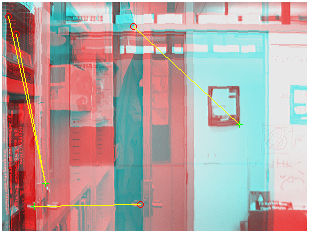
\includegraphics[width=0.8\linewidth]{Images/01_matlab_match.png}
	\caption{Interesting points and matches found using MATLAB's implementation on Image 1.}
	\label{fig:jp-ofc-matlab-match}
\end{figure}

\begin{figure}[H]\centering
	
\includegraphics[width=0.8\linewidth]{Images/01_matlab_depth.png}
	\caption{Depth map using the interesting points and matches using MATLAB's implementation on Image 1.}
	\label{fig:jp-ofc-matlab-depth}
\end{figure}

\begin{figure}[H]\centering
	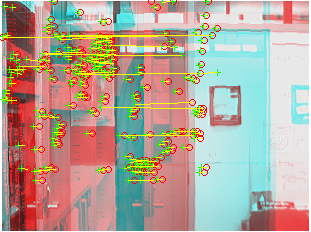
\includegraphics[width=0.8\linewidth]{Images/01_our_match.png}
	\caption{Interesting points and matches using our implementation on Image 1.}
	\label{fig:jp-ofc-ours-match}
\end{figure}

\begin{figure}[H]\centering
	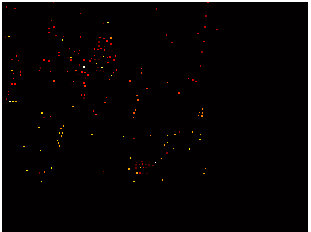
\includegraphics[width=0.8\linewidth]{Images/01_our_depth.png}
	\caption{Depth map using the interesting points and matches using our implementation on Image 1.}
	\label{fig:jp-ofc-ours-depth}
\end{figure}

% Image 2
\begin{figure}[H]\centering
	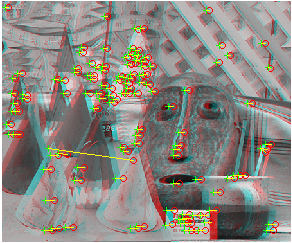
\includegraphics[width=0.8\linewidth]{Images/02_matlab_match.png}
	\caption{Interesting points and matches found using MATLAB's implementation on Image 2.}
	\label{fig:cones-matlab-match}
\end{figure}

\begin{figure}[H]\centering
	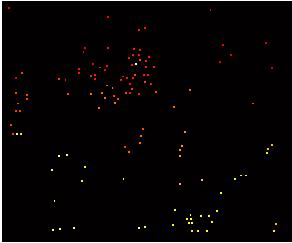
\includegraphics[width=0.8\linewidth]{Images/02_matlab_depth.png}
	\caption{Depth map using the interesting points and matches using MATLAB's implementation on Image 2.}
	\label{fig:cones-matlab-depth}
\end{figure}

\begin{figure}[H]\centering
	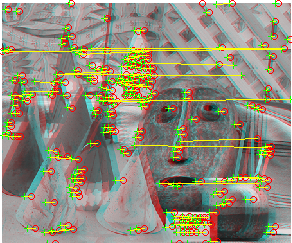
\includegraphics[width=0.8\linewidth]{Images/02_our_match.png}
	\caption{Interesting points and matches using our implementation on Image 2.}
	\label{fig:cones-ours-match}
\end{figure}

\begin{figure}[H]\centering
	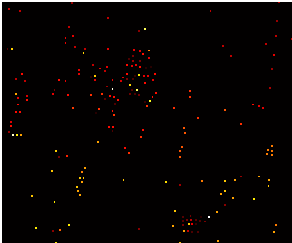
\includegraphics[width=0.8\linewidth]{Images/02_our_depth.png}
	\caption{Depth map using the interesting points and matches using our implementation on Image 2.}
	\label{fig:cones-ours-depth}
\end{figure}

% Image 3
\begin{figure}[H]\centering
	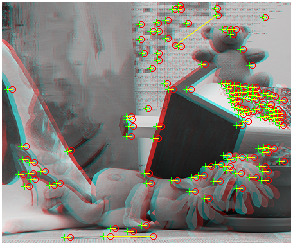
\includegraphics[width=0.8\linewidth]{Images/03_matlab_match.png}
	\caption{Interesting points and matches found using MATLAB's implementation on Image 3.}
	\label{fig:bear-matlab-match}
\end{figure}

\begin{figure}[H]\centering
	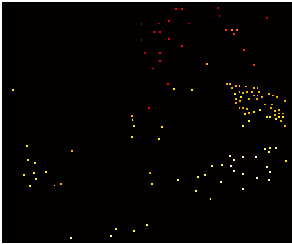
\includegraphics[width=0.8\linewidth]{Images/03_matlab_depth.png}
	\caption{Depth map using the interesting points and matches using MATLAB's implementation on Image 3.}
	\label{fig:bear-matlab-depth}
\end{figure}

\begin{figure}[H]\centering
	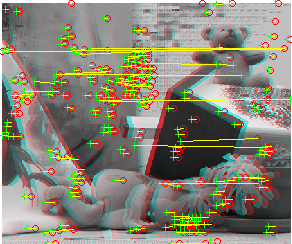
\includegraphics[width=0.8\linewidth]{Images/03_our_match.png}
	\caption{Interesting points and matches using our implementation on Image 3.}
	\label{fig:bear-ours-match}
\end{figure}

\begin{figure}[H]\centering
	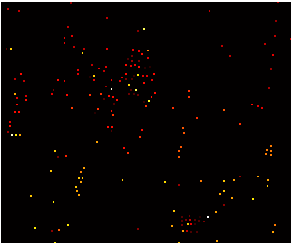
\includegraphics[width=0.8\linewidth]{Images/03_our_depth.png}
	\caption{Depth map using the interesting points and matches using our implementation on Image 3.}
	\label{fig:bear-ours-depth}
\end{figure}

While we had to settle for our fallback goal of creating only a partial depth map, we do believe that our approach showed some merit. Above are shown some examples of our point matching compared with MATLAB's, which uses a 11$\times$11 window as per MATLAB's documentation, and the same depth mapping applied to the results of each set. As you can see in these, our implementation compares reasonably well with MATLAB given the same corner data. This is especially true for the image used in Figures \ref{fig:jp-ofc-matlab-match}-\ref{fig:jp-ofc-ours-depth}, as our algorithm performed exceptionally better than MATLAB, (which actually produced no valid correlations). We assume that this is because of the assumption we make that a match point will lie within a 10-pixel band of its source, allowing us to make more forgiving matches in the case of harsher perspective shifts between the two images.

MATLAB's point correlation did tend to produce smoother depth maps for images with only minor differences however, whereas our implementation introduced substantial noise. This noise is particularly apparent in images like \ref{fig:cones-ours-depth}, with scattered bright spots near the middle. However, the general trend of closer foreground objects toward the bottom images and farther background images toward the top is consistent with what we expect. Our algorithm also had the tendency to make matches that went completely across the image, which we dealt with by discarding outliers above two standard deviations. However, even with this weighting, it simply turned out that these matches were the best that the algorithm could find -- likely a result of being a greedy algorithm and just matching whatever points were left over.  Another possible reason for poor matches in our algorithm, theoretically, is that the corners found in each image may not necessarily be the same.
